%% LyX 1.3 created this file.  For more info, see http://www.lyx.org/.
%% Do not edit unless you really know what you are doing.
\documentclass[english,12pt,a4paper,twoside]{book}
\usepackage{times}
%\usepackage{algorithm2e}
\usepackage{url}
\usepackage{bbm}
\usepackage[T1]{fontenc}
\usepackage[latin1]{inputenc}
\usepackage{geometry}
%\geometry{verbose,letterpaper,tmargin=2.5cm,bmargin=3cm,lmargin=3cm,rmargin=3cm}
\usepackage{rotating}
\usepackage{graphicx}
\usepackage{amsmath, amsthm, amssymb}
\usepackage{setspace}
\usepackage{lineno}
\usepackage{hyperref}
\usepackage{bbm}
\usepackage{pdfpages}

%\usepackage{xcolor,framed}
%\colorlet{shadecolor}{blue!10}
%\begin{shaded}blabla\end{shaded}

%\usepackage{xr}
%\externaldocument{PRS-supp}

%\linenumbers
%\doublespacing
\onehalfspacing
\usepackage[authoryear]{natbib}
%\usepackage{natbib}
%\usepackage{chapterbib}

\usepackage{numprint}
\npthousandsep{,}

%Pour les rajouts
\usepackage{xcolor}

\usepackage{dsfont}
\usepackage[warn]{textcomp}
\usepackage{adjustbox}
\usepackage{multirow}
\usepackage{graphicx}
\graphicspath{{figures/}}
\DeclareMathOperator*{\argmin}{\arg\!\min}

\let\tabbeg\tabular
\let\tabend\endtabular
\renewenvironment{tabular}{\begin{adjustbox}{max width=0.75\textwidth}\tabbeg}{\tabend\end{adjustbox}}

\makeatletter

\usepackage{afterpage}

\newcommand\blankpage{%
    \null
    \thispagestyle{empty}%
    \addtocounter{page}{-1}%
    \newpage}

%%%%%%%%%%%%%%%%%%%%%%%%%%%%%% LyX specific LaTeX commands.
%% Bold symbol macro for standard LaTeX users
%\newcommand{\boldsymbol}[1]{\mbox{\boldmath $#1$}}

%% Because html converters don't know tabularnewline
\providecommand{\tabularnewline}{\\}
\definecolor{clumping}{HTML}{38761D}
\definecolor{thresholding}{HTML}{1515FF}
%<span style="color:#38761D">Clumping</span> + <span style="color:#1515FF">Thresholding</span>

\usepackage{babel}
\makeatother


\begin{document}

\includepdfset{offset=.15in 0in,noautoscale,scale=1,pages={-},pagecommand={}}
\includepdf{cover}

\afterpage{\blankpage}


\clearpage

\section*{Abstract}

Genotyping is becoming cheaper, making genotype data available for millions of individuals.
Moreover, imputation enables to get genotype information at millions of loci capturing most of the genetic variation in the human genome.
Given such large data and the fact that many traits and diseases are heritable (e.g.\ 80\% of the variation of height in the population can be explained by genetics), it is envisioned that predictive models based on genetic information will be part of a personalized medicine.

In my thesis work, I focused on improving predictive ability of polygenic models.
Because prediction modeling is part of a larger statistical analysis of datasets, I developed tools to allow flexible exploratory analyses of large datasets, which consist in two R/C++ packages described in the first part of my thesis.
Then, I developed some efficient implementation of penalized regression to build polygenic models based on hundreds of thousands of genotyped individuals.
Finally, I improved the ``clumping and thresholding'' method, which is the most widely used polygenic method and is based on summary statistics that are widely available as compared to individual-level data.

Overall, I applied many concepts of statistical learning to genetic data. I used extreme gradient boosting for imputing genotyped variants, feature engineering to capture recessive and dominant effects in penalized regression, and parameter tuning and stacked regressions to improve polygenic prediction.
Statistical learning is not widely used in human genetics and my thesis is an attempt to change that.


\clearpage

\section*{R\'esum\'e}

Le g\'enotypage devient de moins en moins cher, rendant les donn\'ees de g\'enotypes disponibles pour des millions d'individus.
Par ailleurs, l'imputation permet d'obtenir l'information  g\'enotypique pour des millions de positions de l'ADN, capturant l'essentiel de la variation g\'en\'etique du g\'enome humain.
Compte tenu de la richesse des donn\'ees et du fait que de nombreux traits et maladies sont h\'er\'editaires (par exemple, la g\'en\'etique peut expliquer 80\% de la variation de la taille dans la population), il est envisag\'e d'utiliser des mod\`eles pr\'edictifs bas\'es sur l'information g\'en\'etique dans le cadre d'une m\'edecine personnalis\'ee.

Au cours de ma th\`ese, je me suis concentr\'e sur l'am\'elioration de la capacit\'e pr\'edictive des mod\`eles polyg\'eniques.
Les mod\`eles pr\'edictifs faisant partie d'une analyse statistique plus large des jeux de donn\'ees, j'ai d\'evelopp\'e des outils permettant l'analyse exploratoire de grands jeux de donn\'ees, constitu\'es de deux packages R/C++ d\'ecrits dans la premi\`ere partie de ma th\`ese.
Ensuite, j'ai d\'evelopp\'e une impl\'ementation efficace de la r\'egression p\'enalis\'ee pour construire des mod\`eles polyg\'eniques bas\'es sur des centaines de milliers d'individus g\'enotyp\'es.
Enfin, j'ai am\'elior\'e la m\'ethode appel\'ee ``clumping and thresholding'', qui est la m\'ethode polyg\'enique la plus largement utilis\'ee et qui est bas\'ee sur des statistiques r\'esum\'ees plus largement accessibles par rapport aux donn\'ees individuelles.

Dans l'ensemble, j'ai appliqu\'e de nombreux concepts d'apprentissage statistique aux donn\'ees g\'en\'etiques. J'ai utilis\'e du ``extreme gradient boosting'' pour imputer des variants g\'enotyp\'es, du ``feature engineering'' pour capturer des effets r\'ecessifs et dominants dans une r\'egression p\'enalis\'ee, et du ``parameter tuning'' et des ``stacked regressions'' pour am\'eliorer les mod\`eles polyg\'eniques pr\'edictifs.
L'apprentissage statistique n'est pour l'instant pas tr\`es utilis\'e en g\'en\'etique humaine et ma th\`ese est une tentative pour changer cela.


\clearpage

\section*{Remerciements}


\clearpage

\tableofcontents


\clearpage

\chapter{Introduction}


\includepdfset{offset=-.25in 0in,noautoscale,scale=0.83,pages={-},pagecommand={}}
%% LyX 1.3 created this file.  For more info, see http://www.lyx.org/.
%% Do not edit unless you really know what you are doing.
\documentclass[english,12pt,a4paper,twoside]{report}
\usepackage{times}
%\usepackage{algorithm2e}
\usepackage{url}
\usepackage{bbm}
\usepackage[T1]{fontenc}
\usepackage[latin1]{inputenc}
\usepackage{geometry}
%\geometry{verbose,letterpaper,tmargin=2.5cm,bmargin=3cm,lmargin=3cm,rmargin=3cm}
\usepackage{rotating}
\usepackage{graphicx}
\usepackage{amsmath, amsthm, amssymb}
\usepackage{setspace}
\usepackage{lineno}
\usepackage{hyperref}
\usepackage{bbm}

%\usepackage{xcolor,framed}
%\colorlet{shadecolor}{blue!10}
%\begin{shaded}blabla\end{shaded}

%\usepackage{xr}
%\externaldocument{PRS-supp}

%\linenumbers
%\doublespacing
\onehalfspacing
%\usepackage[authoryear]{natbib}
\usepackage{natbib} \bibpunct{(}{)}{;}{author-year}{}{,}


%Pour les rajouts
\usepackage{xcolor}

\usepackage{dsfont}
\usepackage[warn]{textcomp}
\usepackage{adjustbox}
\usepackage{multirow}
\usepackage{graphicx}
\graphicspath{{figures/}}
\DeclareMathOperator*{\argmin}{\arg\!\min}

\let\tabbeg\tabular
\let\tabend\endtabular
\renewenvironment{tabular}{\begin{adjustbox}{max width=0.75\textwidth}\tabbeg}{\tabend\end{adjustbox}}

\makeatletter

%%%%%%%%%%%%%%%%%%%%%%%%%%%%%% LyX specific LaTeX commands.
%% Bold symbol macro for standard LaTeX users
%\newcommand{\boldsymbol}[1]{\mbox{\boldmath $#1$}}

%% Because html converters don't know tabularnewline
\providecommand{\tabularnewline}{\\}
\definecolor{clumping}{HTML}{38761D}
\definecolor{thresholding}{HTML}{1515FF}
%<span style="color:#38761D">Clumping</span> + <span style="color:#1515FF">Thresholding</span>

\usepackage{babel}
\makeatother


\begin{document}

\section{Introduction}

In my thesis work, we have been focusing on assessing someone's risk of disease based on DNA data. Except for somatic mutations, DNA data do not change over lifetime so that we could, in theory, assess someone's genetic risk of disease at birth. Thus, this could have potentially large implications in disease prevention \cite[]{mavaddat2015prediction,pashayan2015implications}.
As an example, about 12\% of women in the general population will develop breast cancer sometime during their lives \cite[]{desantis2016breast}. By contrast, a recent large study estimated that about 72\% (95\% CI: 65\%-79\%) of women who inherit a harmful BRCA1 mutation and about 69\% (95\% CI: 61\%-77\%) of women who inherit a harmful BRCA2 mutation will develop breast cancer by the age of 80 \cite[]{kuchenbaecker2017risks}. 
In 2013, Angelina Jolie announced that she had undergone a preventative double mastectomy, because she had a family history of breast cancer and was carrying a harmful BRCA1 mutation.
Thereby, DNA data can help identify individuals who are at high-risk for some diseases in order to target preventive actions.

In this introduction, we first introduce the context of our research and the type of data we work with. Then, we present the statistical methods that are widely used in our field, and how the field has moved from association testing to prediction. Finally, we present the main statistical and computational challenges that has driven our research, which has resulted in two peer-reviewed papers and another submitted paper currently available as a preprint.

\subsection{Context}

Today, clinical risk prediction for common adult-onset diseases often relies on basic demographic characteristics, such as age, gender and ethnicity; basic health parameters and lifestyle factors, such as body mass index, smoking status, alcohol consumption and physical exercise habits; measurement of clinical risk factors linked to disease onset, such as blood pressure levels, blood chemistries or biomarkers indicative of ongoing disease processes; ascertainment of environmental exposures, such as air pollution, heavy metals and other environmental toxins; and family history \cite[]{torkamani2018personal}.
Routine genetic profiling is absent from this list, often relegated to use only when testing clarifies individual-level risks in the context of a known family history for some common adult-onset
diseases \cite[]{torkamani2018personal}.

\subsubsection{Different types of diseases and mutations}

How mutations affect diseases depends on their effect sizes and on their allele frequencies (Figure \ref{fig:rare-common}).
For example, harmful BRCA mutations are highly penetrant mutations, i.e.\ that most women carrying these mutations will develop breast cancer. Many mutations with large effect sizes have been identified and are referenced in an online database \cite[]{hamosh2005online}. 
Those mutations are often very rare; either they are associated with some very rare disease or they explain only a small proportion of common diseases incidence \cite[]{anglian2000prevalence}.
In this work, we focus on common diseases (e.g.\ breast cancer) and try to predict individuals' disease susceptibility based on common variants; the common disease--common variant hypothesis \cite[]{pritchard2002allelic}. This hypothesis further suggests that such diseases are likely caused by a large number of common variants, each contributing only a small risk and thereby evading negative evolutionary selection \cite[]{salari2012personalized}.
Indeed, selection might be responsible for keeping genetic effect sizes low, since variants of larger effect may be selected against and eventually disappear \cite[]{pritchard2002allelic}.
One common form of variation across human genomes is called a single nucleotide polymorphism (SNP). As indicated by the name, SNPs are single base changes in the DNA.
Genotyping technologies now exists to genotype hundreds of thousands of SNPs at once for around \$50 only. Starting with the \cite{wellcome2007genome}, these new sequencing technologies had led to many genome-wide association studies.%, which we talk about in the next section. From these studies, it was found that effects of common variants that are associated with some disease are typically very small.

\begin{figure}[htb]
\centerline{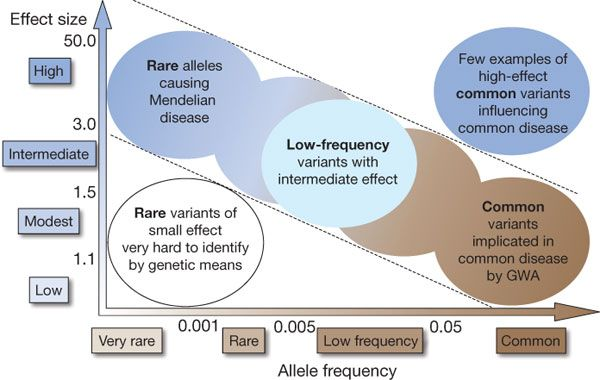
\includegraphics[width=0.7\textwidth]{rare-common.jpg}}
\caption{Feasibility of identifying genetic variants by risk allele frequency and strength of genetic effect (odds ratio). Most emphasis and interest lies
in identifying associations with characteristics shown within diagonal dotted
lines. Source: \cite{manolio2009finding}.}
\label{fig:rare-common}
\end{figure}

\subsubsection{Genome-Wide Association Studies (GWAS)}

\cite{visscher201710} provide a thorough review of the aims and outcomes of GWAS and \cite{tam2019benefits} talk extensively about the benefits and limitations of GWAS.
The method behind GWAS is simple: test each variant one by one for association with a phenotype of interest.
For a continuous phenotype (e.g.\ height), linear regression is used and, for each SNP $j$, a t-test is performed to look for an association between this SNP and the phenotype of interest ($\beta^{(j)} = 0$ vs $\beta^{(j)} \neq 0$), where
\begin{equation}
y = \alpha_j + \beta_j G_{j} + \gamma_j^{(1)} COV^{(1)} + \cdots + \gamma_j^{(K)} COV^{(K)} + \epsilon~,\label{eq:gwas1}
\end{equation}
$y$ is the continuous phenotype, $\alpha_j$ is the intercept, $G_{j}$ is SNP $j$ with effect $\beta_j$, $COV^{(1)}$, ..., $COV^{(K)}$ are $K$ covariates with effects $\gamma_j^{(1)}$, ..., $\gamma_j^{(K)}$, including principal components and other covariates such as age and gender. Similarly, for a binary phenotype (e.g.\ disease status), logistic regression is used and a Z-test is performed on $\beta^{(j)}$ for each SNP $j$ where
\begin{equation}
\log{\left(\frac{p}{1-p}\right)} = \alpha_j + \beta_j G_{j} + \gamma_j^{(1)} COV^{(1)} + \cdots + \gamma_j^{(K)} COV^{(K)}~,\label{eq:gwas2}
\end{equation}
$p = \mathbb{P}(Y = 1)$ and $Y$ denotes the binary phenotype.

It is well established that principal components of genotype data should be included as covariates in GWAS to account for the confounding effect of population structure \cite[]{price2006principal}. Indeed, principal components of genotype data capture well population structure (as shown in figure \ref{fig:pca}). 
To illustrate the importance of accounting for population structure, consider a dataset where there are 900 Finnish people and 100 Italian people. Because Finnish people are on average taller than Italian people, any SNP with a large difference in allele frequency between these two populations would be flagged as being associated with height, leading to many false positive associations. Thus, adding principal components as covariates aims at preventing those SNPs from being false positive reports.

\begin{figure}[htb]
\centerline{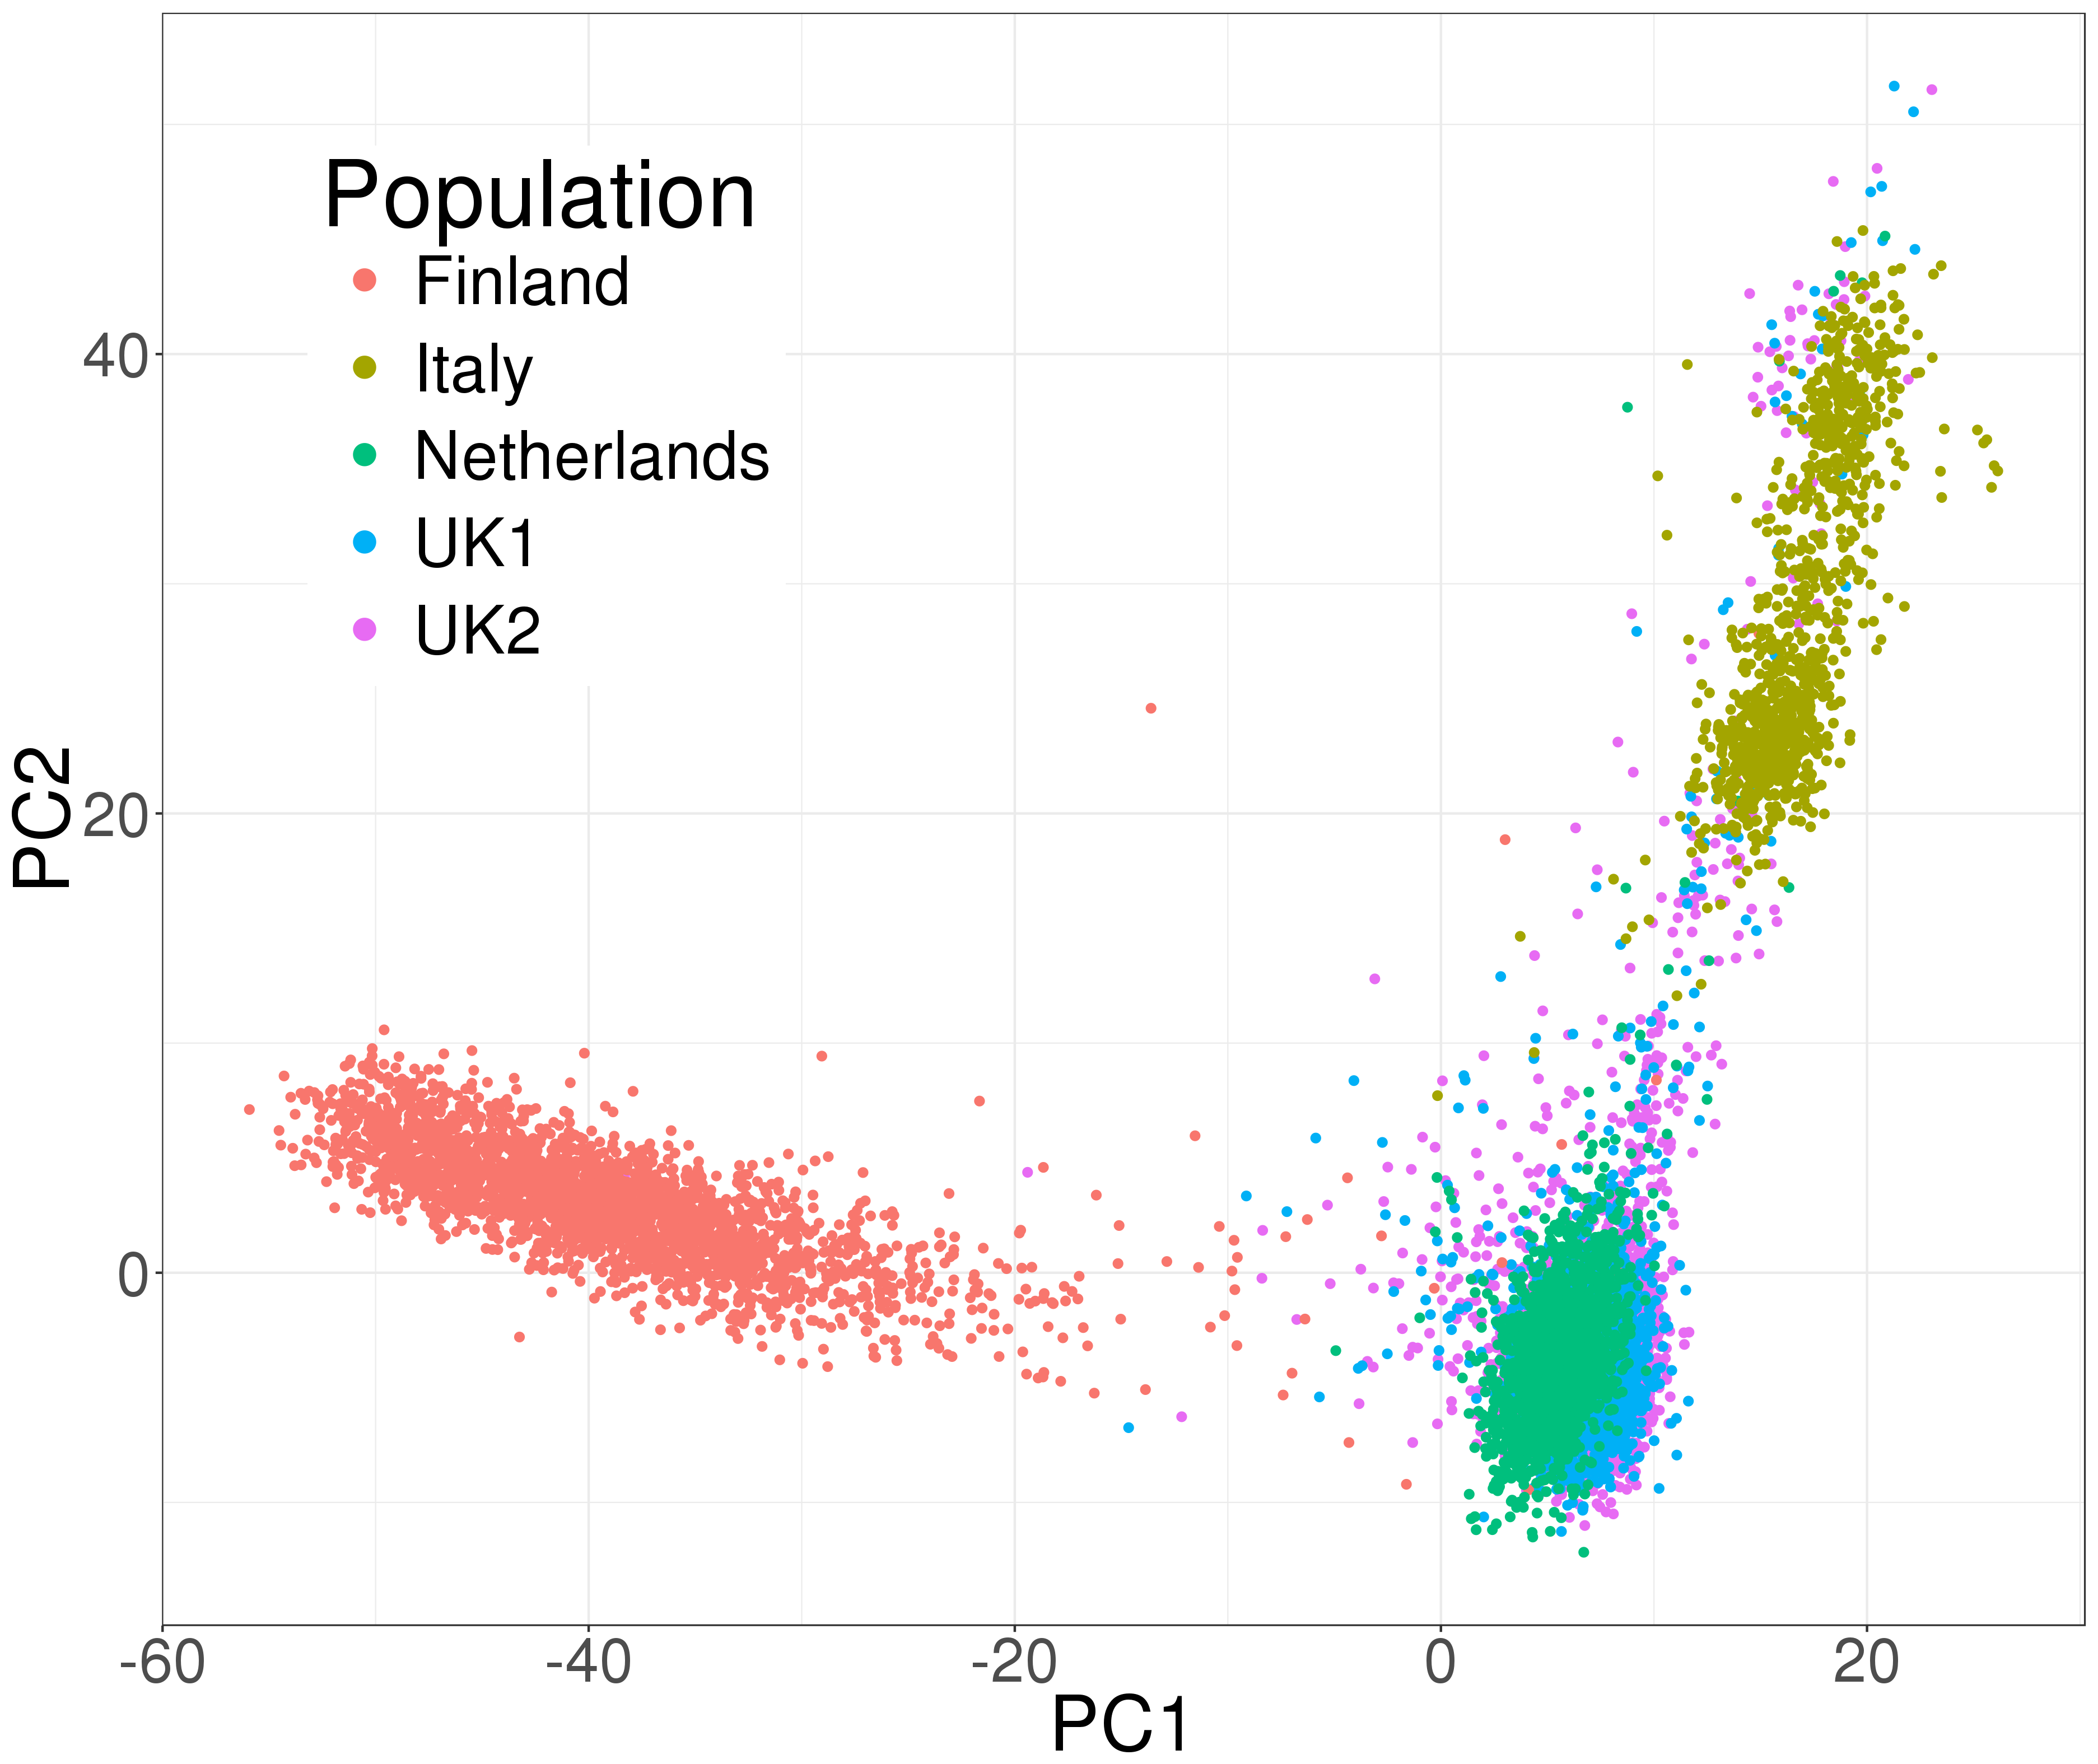
\includegraphics[width=0.6\textwidth]{celiac-pca.png}}
\caption{First two Principal Components of individuals from four European populations. PC1 correlates with latitude while PC2 correlates longitude. Data come from a case-control study for celiac disease \cite[]{dubois2010multiple}.}\label{fig:pca}
\end{figure}

These simple tests can be used only if individuals are not related to one another. If they do, a common practice is to remove one individual from each pair of related individuals. Another strategy is to use Linear Mixed Models (LMM) to take into account both relatedness and population structure; these mixed models have also the potential to increase discovery power in association testing \cite[]{yang2014advantages}.

To date, more than 10,000 strong associations have been reported between genetic variants and one or more complex traits \cite[]{welter2013nhgri}, where ``strong'' is defined as statistically significant at the genome-wide p-value threshold of $5 \cdot 10^{-8}$. This threshold corresponds to a type-I error of 5\%, Bonferroni-corrected for one million independent tests \cite[]{pe2008estimation}. Results of a GWAS are usually reported in a Manhattan plot (Figure \ref{fig:gwas}). 
Manhattan plots show some association peaks (similar to skyscrapers in Manhattan) due to some local correlation between SNPs (Linkage Disequilibrium), with squared correlation roughly inversely proportional to distance between SNPs \cite[]{hudson2001two}.

\begin{figure}[htb]
\centerline{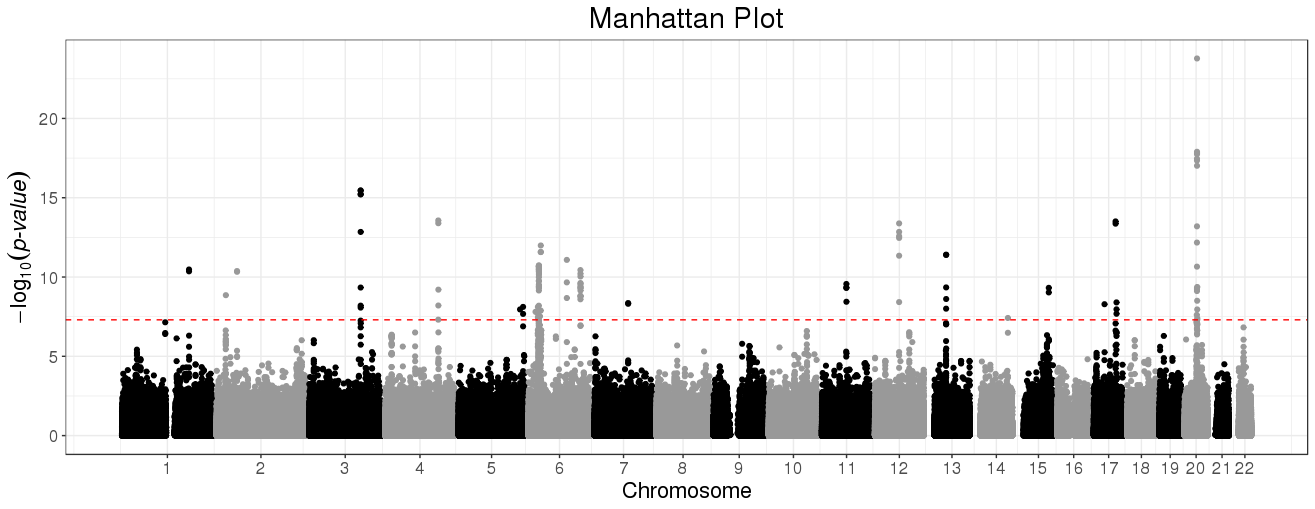
\includegraphics[width=0.95\textwidth]{gwas-height-20K.png}}
\caption{Manhattan plot from a GWAS of height based on 20,000 unrelated individuals from the UK Biobank dataset \cite[]{bycroft2017genome}.}\label{fig:gwas}
\end{figure}


\subsubsection{GWAS data}

There are mainly three types of individual-level data: genotyped SNPs from genotyping chips, imputed SNPs from reference panels, and Next Generation Sequencing (NGS) data.
Genotyping chips enables a quick and cheap genotyping of 200K to 2M SNPs, mostly focusing on common variants (Minor Allele Frequency (MAF) larger than 1-5\%). From this genotyping, you can get a matrix of $0$s, $1$s and $2$s, counting the number of alternative alleles for each individual (row) and each genome position (column). There are usually few missing values (less than 5\% in total) when using this technology.

Imputation has a different meaning in genetics than in other Data Science fields; it does not refer to filling those 5\% missing values, but instead refers to adding completely new variants that were not genotyped with the chip used. 
Imputation is enabled by the fact that genotypes of unobserved genetic variants can be predicted by haplotypes inferred from multiple observed SNPs (the ones that were genotyped) and haplotypes observed from a fully sequenced reference
panel \cite[]{marchini2010genotype,mccarthy2016reference}.
Imputation now allows to have large genomic datasets such as the UK Biobank: 90M imputed SNPs for each of 500K genotyped individuals who were sequenced at 800K SNPs only \cite[]{bycroft2017genome}.

Finally, NGS (also named Whole Genome Sequencing (WGS)) refers to fully sequenced data over more than 3M variants, including some rare variants. Yet, this technology is still very expensive, with a cost of around \$1000 per genome.
GWAS to date have been based on SNP arrays designed to tag common variants in the genome. These arrays do not cover all genetic variants in the population, and it seems natural that future GWAS will be based on WGS. However, the price differential between SNP arrays and WGS is still substantial, and array technology remains more robust than sequencing \cite[]{visscher201710}. An in-between solution could be to use extremely low-coverage sequencing \cite[]{pasaniuc2012extremely}.

Recently, some national biobank projects have emerged. For example, the UK Biobank has released both genome-wide genotypes and rich phenotypic data on 500K individuals to the international research community \cite[]{bycroft2017genome}.
Yet, it is rare to have access to large individual-level genotype data. 
Most of the time, only summary statistics for a GWAS dataset are available, i.e.\ the estimated effect sizes and p-values for each variant of the dataset (Table \ref{tab:sumstats}). Because of the availability of such data en masse, specific methods using those summary data have been developed for a wide range of applications such as imputation, polygenic prediction and heritability estimation \cite[]{pasaniuc2014fast,vilhjalmsson2015modeling,bulik2015ld,pasaniuc2017dissecting,speed2018sumher}. The craze for such data can be explained by the fact that GWAS individual-level data, sometimes consisting of dozens of different datasets, cannot be easily shared publicly, as opposed to summary data \cite[]{lin2010meta}.
So, modern large GWAS are in fact meta-analyses of many smaller GWAS summary statistics.
Moreover, methods using summary statistics data are usually fast and easy to use, making them even more appealing to researchers.

In this thesis, we have not used NGS data, but we have used genotyped SNPs, imputed SNPs and summary statistics to construct predictive models of disease risk, for many common diseases.

% latex table generated in R 3.5.2 by xtable 1.8-2 package
% Wed Apr  3 17:55:25 2019
\begin{table}[ht]
\caption{An example of summary statistics for type 2 diabetes \cite[]{scott2017expanded}. Generally, effects and p-values are available for all SNPs in the GWAS, where there can be many millions of them \cite[]{asking4more}.}\label{tab:sumstats}
\vspace{0.5em}
\centering
\begin{tabular}{rrccrrrr}
  \hline
Chr & Position & Allele1 & Allele2 & Effect & StdErr & P-value & TotalSampleSize \\ 
  \hline
   5 & 29439275 & T & C & -0.000 & 0.015 & 0.990 & 111309 \\ 
     5 & 85928892 & T & C & -0.008 & 0.031 & 0.790 & 111309 \\ 
    11 & 107819621 & A & C & -0.110 & 0.200 & 0.590 & 87234 \\ 
    10 & 128341232 & T & C & 0.024 & 0.015 & 0.110 & 111309 \\ 
     8 & 66791719 & A & G & 0.069 & 0.120 & 0.560 & 99092 \\ 
    23 & 145616900 & A & G & -0.011 & 0.060 & 0.860 & 19870 \\ 
     3 & 62707519 & T & C & 0.006 & 0.034 & 0.860 & 111308 \\ 
     2 & 80464120 & T & G & 0.110 & 0.057 & 0.062 & 108514 \\ 
    18 & 51112281 & T & C & -0.011 & 0.016 & 0.490 & 111307 \\ 
     1 & 209652100 & T & C & 0.260 & 0.170 & 0.120 & 84836 \\ 
   \hline
\end{tabular}
\end{table}


%%%%%%%%%%%%%%%%%%%%%%%%%%%%%%%%%%%%%%%%%%%%%%%%%%%%%%%%%%%%%%%%%%%%%%%%%%%%%%%%


\subsection{From GWAS to Polygenic Risk Scores (PRS)}

For thorough guides on how to perform PRS analyses, please refer to \cite{wray2014research,chasioti2019progress,choi2018guide}.

\subsubsection{A standard way to compute PRS}\label{sec:C+T}

The main method for computing Polygenic Risk Scores (PRS) is the widely used ``Clumping + Thresholding'' (C+T, also called ``Pruning + Thresholding'' in the literature) model based on univariate GWAS summary statistics as described in equations \eqref{eq:gwas1} and \eqref{eq:gwas2}.
Under the C+T model, a coefficient of regression is learned independently for each SNP along with a corresponding p-value (the GWAS part). 

The SNPs are first clumped (C) so that there remains only SNPs that are weakly correlated with each other ($S_\text{clumping}$). Clumping looks at the most significant SNP first, computes correlation between this index SNP and nearby SNPs (within a genetic distance of e.g.\ 500kb) and remove all the nearby SNPs that are correlated with this index SNP beyond a particular threshold (e.g.\ $r^2 = 0.2$, \cite{wray2014research}). 
The clumping step aims at removing redundancy in included effects that is simply due to linkage disequilibrium (LD) between variants (see figures \ref{fig:gwas2} and \ref{fig:gwasLD}). Yet, this procedure may as well remove independently predictive variants in nearby regions.

Thresholding (T) consists in removing SNPs that are under a chosen level of significance (a p-value threshold $p_T$) in order to reduce noise in the score.
In figure \ref{fig:gwas2}, using no threshold corresponds to ``C+T-all''; using the genome-wide threshold of $5 \cdot 10^{-8}$ corresponds to ``C+T-stringent''; generally, many values are tested to choose an ``optimal'' value for this parameter. 

A polygenic risk score is finally defined as the sum of allele counts of the remaining SNPs (after clumping and thresholding) weighted by the corresponding GWAS effect sizes \cite[]{purcell2009common,Dudbridge2013,wray2014research,Euesden2015},
\[\rm{PRS}_i = \sum_{\substack{j \in S_\text{clumping} \\ p_j~<~p_T}} \hat\beta_j \cdot G_{i,j}~,\] where $\hat\beta_j$ ($p_j$) are the effect sizes (p-values) estimated from the GWAS and $G_{i,j}$ is the allele count (genotype) for individual $i$ and SNP $j$.

\begin{figure}[htb]
\centerline{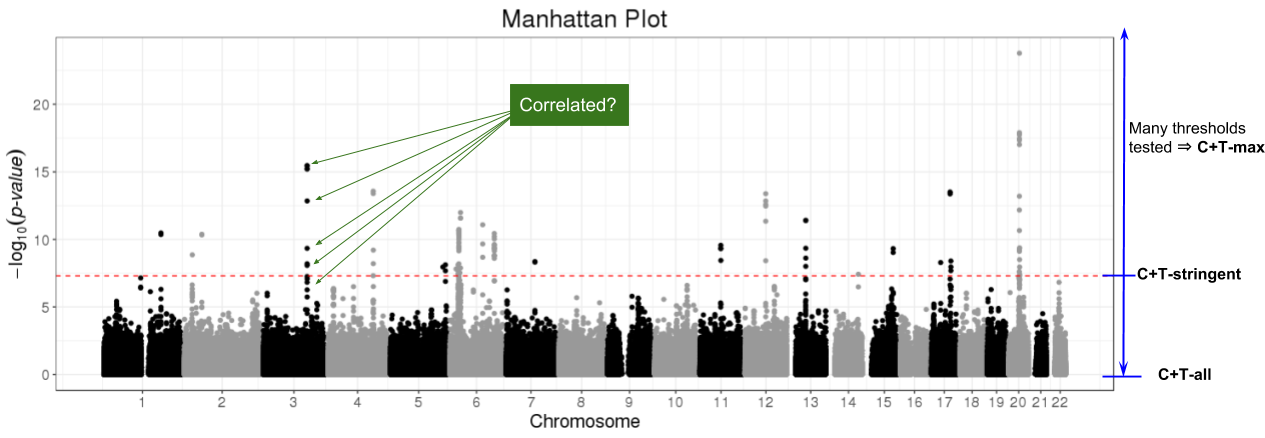
\includegraphics[width=0.95\textwidth]{GWAS2PRS3.png}}
\caption{Illustration of C+T looking at a Manhattan plot from a GWAS of height based on 20,000 unrelated individuals from the UK Biobank dataset \cite[]{bycroft2017genome}. \textbf{\color{clumping}Clumping} removes nearby SNPs that are too correlated with one another because indirect associations due to Linkage Disequilibrium provide only redundant information (see figure \ref{fig:gwasLD}). \textbf{\color{thresholding}Thresholding} includes SNPs if they are significant enough ($p_j < p_T$) in order to reduce noise in the polygenic score.}\label{fig:gwas2}
\end{figure}

\begin{figure}[htb]
\centerline{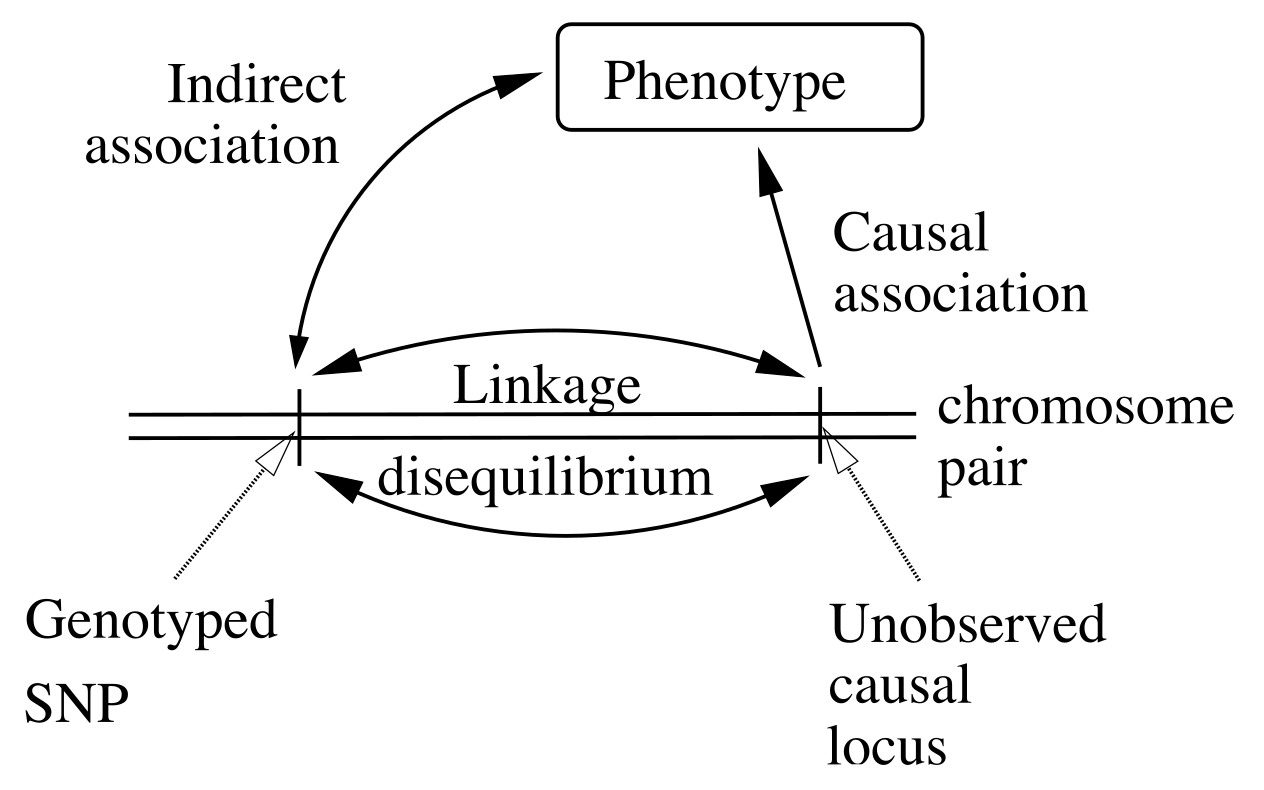
\includegraphics[width=0.5\textwidth]{indirect-association.png}}
\caption{Illustration of an indirect association with a phenotype due to Linkage Disequilibrium between SNPs. Source: \cite{astle2009population}.}\label{fig:gwasLD}
\end{figure}

\subsubsection{PRS for epidemiology}

Polygenic Risk Scores (PRS) have been used for epidemiology before being used for prediction. The steps for a PRS analysis are illustrated in figure \ref{fig:steps-PRS} and have two goals. 
First, PRS can be used when there is no SNP detected (at $5 \cdot 10^{-8}$) in a GWAS in order to show that there is still a significant polygenic contribution to the phenotype of interest. 
For example, in 2009, a GWAS for Schizophrenia by \cite{purcell2009common} found only a single significantly associated SNP, although this disease is known to be highly heritable. Yet, by constructing a PRS using these GWAS results and testing this polygenic score for association with Schizophrenia in another independent dataset, \cite{purcell2009common} proved that there is a polygenic contribution to Schizophrenia (Figure \ref{fig:epi-PRS}). 
Thus, polygenic analysis methods were central in demonstrating that the first phase of GWAS were underpowered, which propelled the drive for larger sample sizes that is now starting to pay off \cite[]{wray2014research}.

\begin{figure}[htb]
\centerline{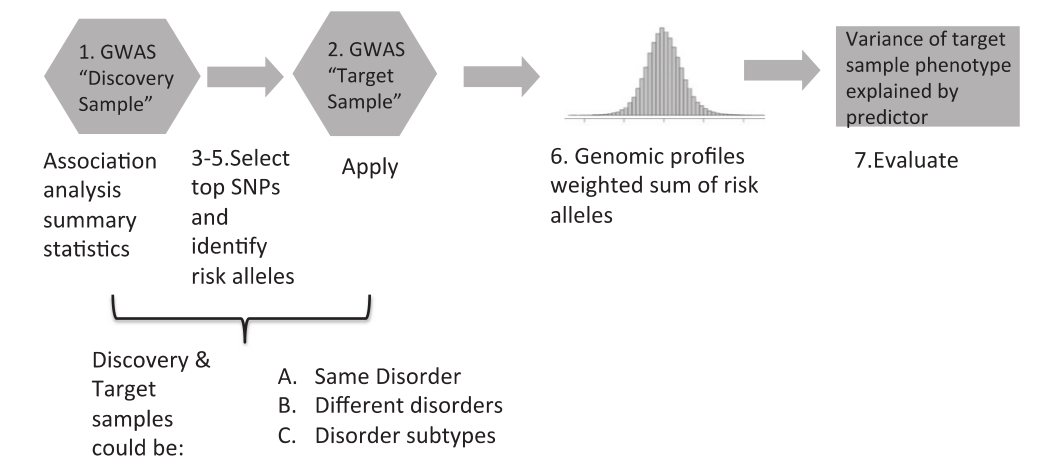
\includegraphics[width=0.8\textwidth]{genomic-profile.png}}
\caption{Illustration of the steps in genomic profile risk scoring. Source: \cite{wray2014research}.}\label{fig:steps-PRS}
\end{figure}

\begin{figure}[htb]
\centerline{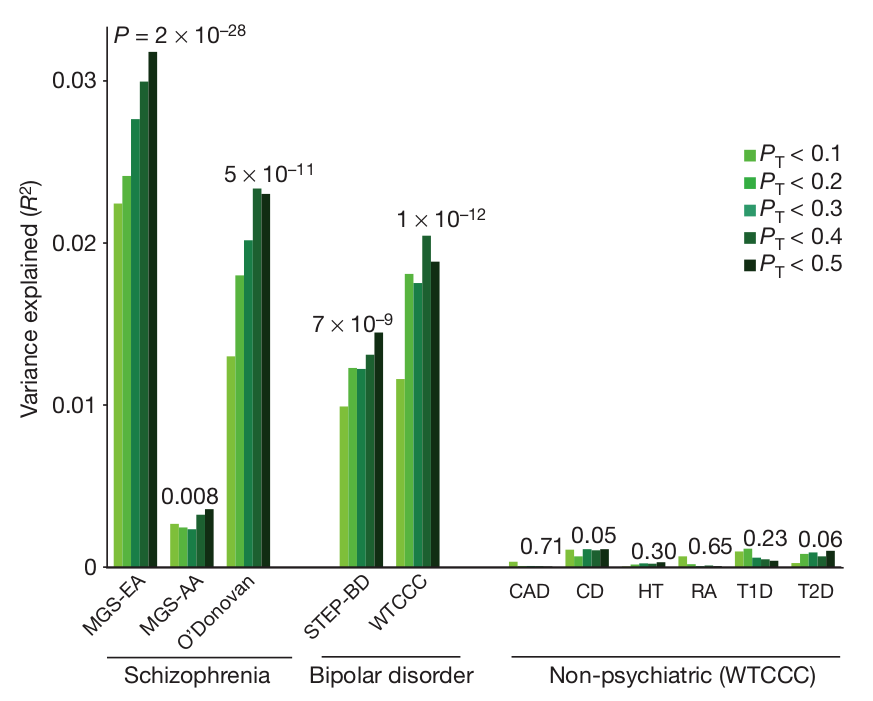
\includegraphics[width=0.65\textwidth]{purcell2009.png}}
\caption{Replication of the polygenic component derived by the International Schizophrenia Consortium in independent schizophrenia and bipolar disorder samples. A PRS was computed using summary statistics from a GWAS of schizophrenia, and this polygenic score was tested for association with schizophrenia, bipolar disorder and other diseases in independent datasets. This proved that there was a polygenic contribution to schizophrenia, a common genetic contribution between schizophrenia and bipolar disorder, but no apparent common genetic contribution between schizophrenia and other diseases such as coronary artery disease, Crohn's disease, hypertension, rheumatoid arthritis and diabetes. Associations were maximized for $p_T = 0.5$, i.e.\ including more than half of all SNPs. Source: \cite{purcell2009common}.}\label{fig:epi-PRS}
\end{figure}

Another use of PRS for epidemiology is to test the PRS for association with a phenotype that is different from the one used to compute the summary statistics.
This technique enables researchers to prove that there is a common genetic contribution between two traits. 
For example, it was shown that there is a common genetic contribution between Schizophrenia and bipolar disorder (Figure \ref{fig:epi-PRS}). 


\subsubsection{The differing goals of association testing and risk prediction}

Association testing (GWAS) and prediction have very different goals.
First, GWAS aims at identifying highly replicable disease-associated variants by using a highly stringent p-value threshold to prevent false discoveries. However, using only hits from GWAS results in PRS of low predictive value (see section \ref{sec:missing}). 
A common mistake is to report highly significant findings with large odds ratios as useful predictors of disease. 
Thus, people have been reminded over the years that GWAS findings are often not predictive on their own even if they are highly associated with the disease of interest, and that we would need scores that combine many SNPs in order to have a decent predictor of disease, i.e.\ polygenic scores \cite[]{pepe2004limitations,janssens2006predictive,jakobsdottir2009interpretation,wald2019illusion}.

Finally, it should be noted that population stratification, usually considered an unwelcome confounder in GWAS, may be useful in risk prediction and may be leveraged to produce better models \cite[]{golan2014effective,abraham2015genomic}.
Indeed, for predictive purposes, the objective is to provide the best possible prediction and confounding is not an issue. However, it might become an issue when polygenic risk scores (PRS) capture population structure in addition to trait variation. For instance, correlation between a PRS and an outcome might be due to residual population structure instead of real genetic contribution to the outcome \cite[]{sohail2019polygenic}.


\subsection{Polygenic prediction}

\subsubsection{Heritability and missing heritability} \label{sec:missing}

The basic components of disease risk are usually broken down into genetic susceptibility, environmental exposures and lifestyle factors. Thus, all disease incidence cannot be predicted by genetic factors only.
For a quantitative phenotype, we call heritability ($h^2$) the proportion of phenotypic variation that is attributable to genetic factors among a population \cite[]{visscher2008heritability}.
Methods now enable the estimation of chip-heritability (also called SNP-heritability: $h^2_{SNP}$) using linear mixed models and residual maximum likelihood. For example, for a chip of 300K SNPs, it was shown that those SNPs could account for 45\% of the variance of height \cite[]{yang2010common}.
Note that the heritability of height is estimated to be around 80\% \cite[]{silventoinen2003determinants,visscher2006assumption}; the difference between these two values can be explained by the fact that 300K SNPs cannot capture the same variation in height as the 3 billion base pairs of DNA. This difference can also reflect an overestimation of heritability \cite[]{visscher2008heritability}. Authors of a recent preprint claim that they can recover the full heritability for height and BMI using both rare and common variants from NGS data \cite[]{wainschtein2019recovery}.

So, basically, heritability is the upper bound in terms of prediction power (when measured with $R^2$) that we can get using a model from genetic variants only.
The difference between $R^2$ and $h^2$ has been termed ``missing heritability'' \cite[]{manolio2009finding}. So, the main goal of genetic prediction and my thesis is to get best possible predictions based on genetic data in order to reduce this missing heritability.

The gap between predictions and heritabilities was really huge in the first years of GWAS.
For example, first GWAS found only 12 associated SNPs for type 2 diabetes and only 2 for prostate cancer, explaining a very small proportion of heritability for these diseases \cite[]{jakobsdottir2009interpretation}. 
Likewise, in 2008, only 40 genome-wide-significant SNPs had been identified for height, and together these explained about 5\% of the heritability of height \cite[]{manolio2009finding}. In 2014, the number of associated SNPs had increased to around 700, explaining 20\% of the heritability of height \cite[]{wood2014defining}.
Since most of the identified associated SNPs have an effect size close to the limit dictated by the power of the studies, a likely explanation, at least in part, is that there are many common polymorphisms with effects that are too small to pass the stringent significance threshold of current GWAS \cite[]{wray2008prediction}.
Therefore, as results from multiple GWAS are combined to increase sample size, a larger fraction of the genetic variance is likely to be explained and accurate prediction of genetic risk to disease will become possible even though the risks conveyed by individual variants are small \cite[]{wray2008prediction,wray2018common}.
These findings have also led people to use not only genome-wide significant SNPs, but many other SNPs, sometimes not even marginally significant (i.e.\ with a p-value > 5\%) in order to maximize predictive power \cite[]{purcell2009common,Dudbridge2013,wray2014research}.


\subsubsection{Methods for polygenic prediction}

Several methods have been developed to predict disease status based on SNP information.
We can divide these methods in two categories: the ones that use summary statistics and the ones that use individual-level data only.

When summary statistics are available, the most widely used method is called ``Clumping + Thresholding'' (C+T), which has been described in section \ref{sec:C+T}.
More recently, researchers have focused their efforts on implementing more elegant and potentially more optimal ways to account for LD, as a replacement of clumping that simply discards SNPs \cite[]{vilhjalmsson2015modeling,mak2017polygenic,chun2019non,ge2019polygenic}. 
Take the solution of a linear regression $y = X \beta + \epsilon$, $\hat{\beta} = \left(X^T X\right)^{-1} X^T y$. This vector of effect sizes $\hat{\beta}$, estimated from all variables at once, can be decomposed in two parts: $X^T y$ that represents the marginal effects, i.e.\ the effects of each variable when learned independently; and $\left(X^T X\right)^{-1}$, some rotation of the effects that account for the correlation between variables.
Then, the first element can be replaced by summary statistics and the second element can be replaced by an estimation of the LD structure of the SNPs, e.g.\ from a reference panel. 
In practice, [$X^T y$ is estimated by TODO] and $\left(X^T X\right)^{-1}$ is computed by window. [TODO: parler de bayesian or lasso]


Moreover, these methods handle weights differently than C+T that directly uses GWAS effect sizes as weights in the PRS, or weights of 0 for SNPs not passing the thresholding step. Instead, these methods usually shrink effects towards 0. 
Apart from the method of \cite{mak2017polygenic}, the other methods do not perform variable selection at all. This means that if you use GWAS summary statistics for 10M variants as input, you would get a predictive model composed of 10M variables \cite[]{janssens2019polygenic}.

When using individual-level data only, the problem boils down to a standard classification problem. Thus, some statistical learning methods have been used to derive PRS for complex human diseases by jointly estimating SNP effects. Such methods include joint logistic regression, Support Vector Machine (SVM) and random forests \cite[]{wei2009disease,abraham2012sparsnp,abraham2014accurate,botta2014exploiting,okser2014regularized}.
Linear Mixed-Models (LMMs) are another widely-used method in fields such as plant and animal breeding or for predicting highly heritable quantitative human phenotypes such as height \cite[]{yang2010common}. 
However, these methods and their derivatives are often computationally very demanding, both in terms of memory and time required \cite[]{zhou2013polygenic,golan2014effective,speed2014multiblup,maier2015joint}.
Recently, two methods named BOLT-LMM and SAIGE have been developed to handle very large datasets \cite[]{loh2018mixed,zhou2018efficiently}. BOLT-LMM and SAIGE were primarily designed for association testing but could also be used for prediction purposes based on individual-level data.

\subsubsection{Objective and main difficulties of the thesis}

We want to use genetic data to help distinguish between cases and controls for a given disease, or at least to stratify people in the population in order to improve early detection of diseases and prevention for high-risk individuals.
Genomic data are usually very large and highly dimensional with hundreds of thousands of variables to many millions, for thousands or hundred of thousands individuals.
Thanks to large sample sizes of recent GWAS studies, many robust associations between DNA variants and many diseases have been identified. Yet, individually, these variants generally have a small effect on disease susceptibility, explaining a small fraction of the total heritability of the diseases studied. 
In order to have predictive models useful in clinical settings, we need to combine the information from a multitude of DNA variants, coming from multiple studies, and in diverse formats (e.g.\ individual-level data and summary statistics).

To improve current disease predictions from Polygenic Risk Scores (PRS), we have focused on using methods from the statistical learning community, which have received only moderate attention in the "predictive human genetics" field.
The main difficulty in using these methods is that they do not necessarily scale well with the large-scale data we now have in this field.
For example, the UK Biobank is composed of 500K individuals from which 90M variants are available \cite{bycroft2017genome}.
When analyzing these large-scale datasets, only a few methods are usable.
Most of them are being developed in a separate piece of software that does a specific analysis.
Yet, if you want to do some exploratory analyses and test new ideas, it becomes increasingly difficult to do so.

Thus, the first part of our work has been dedicated to developing two R packages that could handle very large datasets, while being simple and flexible to use for both standard and exploratory analyses. 
Our second paper has been dedicated to implementing penalized regressions as a replacement to more simple, less optimal methods, and that could be used for very large individual-level datasets.
Finally, because lots of summary statistics data are available while individual-level data are still scarce, we worked on making the most out of the Clumping and Thresholding (C+T) method since it proved to be a simple and effective method for constructing PRS based on large GWAS summary statistics and smaller individual-level datasets.

%[COMPLETER]

\newpage

\bibliographystyle{natbib}
\bibliography{refs}

\end{document}



\chapter[R packages for analyzing genome-wide data]{Efficient analysis of large-scale genome-wide data with two R packages: bigstatsr and bigsnpr}

\section{Summary of the article}

\subsection{Introduction}

Sample size of GWAS data has rapidly grown due to the reduction in genotyping costs over the years. Moreover, thanks to the imputation of many non-genotyped SNPs, the number of available SNPs for a given dataset has grown to millions. In 2007, there were datasets with 2000 cases and 3000 controls, genotyped over 300K SNPs \cite[]{wellcome2007genome}. Now, there are datasets of 500K individuals, genotyped over 800K SNPs, and imputed over 90M SNPs \cite[]{bycroft2017genome}.
Genotype data are the first data of the omics family to have grown to such large scale. To analyze these datasets, software have been consistently produced or updated over the years in order to keep up with growing sizes. 
I think this is one rare field where producing software is really recognized as an important part of research to help advance the field.
An obvious example in genetics is PLINK, a command line software whose first version has been cited more than 17K times since 2007 and whose second version has already been cited more than 1500 times since 2015 \cite[]{purcell2007plink,chang2015second}. This software is useful for file conversions as well as many types of analyses and is used in plant, animal and human genetics alike.

I wanted to use R to analyze data from this field as it provides excellent tools for exploratory analyses. 
R is a programming language that makes it easy to tie together existing or
new functions to be used as part of large, interactive and reproducible
analyses \cite[]{R2018}.
Yet, most of the R packages that have been developed in Human Genetics are now obsolete because they cannot scale to the size of the data we currently have in the field.
The first problem there is to solve is to actually store the data. For example, a standard R matrix of size 500K x 800K would require 3TB of RAM just to access it in memory.
The second problem is the computation time; if all functions provided by a package take two weeks to run, it is not really useful.

\subsection{Methods}

We developed two R packages called bigstatsr and bigsnpr. 
To solve the memory issue, we use a data format stored as a binary file on disk but that can be accessed almost as if it were a standard R matrix. 
To provide functions with a reasonable computation time, I spent thousands of hours on the performance of code. Moreover, most of the functions provided in these packages are parallelized, which is facilitated by the fact that the data is stored on disk, therefore accessible by each process without the need of any copying.
The R packages makes extensive uses of some C++ code in order to fully optimized key parts of the provided functions.

Specifically, package bigstatsr provides the on-disk data format and some standard statistical algorithms such as Principal Component Analysis (PCA), multiple association testing, matrix products, etc. for this type of data. 
This package is not specific to genetic data and can be used by other fields of Research.
Package bigsnpr builds on top of package bigstatsr and provides algorithms specific to GWAS data. It also provides wrappers to commonly-used software such as PLINK in order to perform all the analysis within R, making it both simple and reproducible\footnote{\url{https://hackseq.github.io/2017\_project\_5/all-in-R.html} \cite[]{grande2018hackathon}}.
To save some disk space and make accesses faster, we store genotype matrices using only  
byte per element, instead of eight bytes per element for a standard R matrix. With a special format, we are able to store both hard calls (0s, 1s, 2s and NAs) and dosages (expected values from imputation probabilities, $d = 0 \times \mathbb{P}(0) + 1 \times \mathbb{P}(1) + 2 \times \mathbb{P}(2)$).

We also developed two new algorithms by building on existing R packages.
One algorithm is used for the imputation of missing values inside a genotype matrix. Generally, there are less than 1\% of missing data in a genotype matrix, and current algorithms for filling these blanks relies on complex inference algorithms. 
Notably, these algorithms rely on a first step of phasing, which consists in inferring haplotypes from genotypes. Phasing is very computationally demanding, so that we propose an algorithm based on XGBoost, an efficient algorithm for building decision trees using extreme gradient boosting, which allows for reconstructing data for one SNP based on non-linear combinations of nearby SNPs.
The other algorithm infer consecutive loadings that capture the structure of long-range LD regions instead of capturing population structure when performing PCA on SNP data.
This new algorithm relies on pcadapt, an algorithm that find outlier loadings in PCA \cite[]{luu2017pcadapt}. 

\subsection{Results}

We show that our two R packages are very efficient and can perform standard analyses as fast as dedicated command-line software such as PLINK, and much faster than previously developed R packages.
We also show that commonly used software for computing principal components of genomic data are not accurate enough in some cases.
Finally, we show that, thanks to our two newly developed algorithms, we are able to quickly impute the few missing values in a genotype matrix while being almost as accurate as more complex and computationally demanding software. We also show that our iterative algorithm to detect and remove long-range LD regions while computing PCA makes it possible to automatically retrieve population structure without capturing any LD structure.

\subsection{Discussion}

We developed two very fast R packages for analyzing large genomic data. One of them, bigstatsr, is not specific to SNP data so that it could be used by other fields of Research that need to analyze large matrices.
Moreover, we think these packages are simple to use, very well tested and easily maintainable because of relatively simple code.
The two R packages use a matrix-like format, which makes it
easy to develop new functions in order to experiment and develop
new ideas. Integration in R makes it possible to take advantage of
the vast and diverse R packages.


\bibliography{refs}

\section{Article and supplementary data}

The following article is published in \textit{Bioinformatics}	\footnote{\url{https://doi.org/10.1093/bioinformatics/bty185}}.

\includepdf[pages=-]{paper1.pdf}
\includepdf[pages=-]{paper1-supp.pdf}



\chapter[Efficient penalized regression for PRS]{Efficient Implementation of Penalized Regression for Genetic Risk Prediction}

%% LyX 1.3 created this file.  For more info, see http://www.lyx.org/.
%% Do not edit unless you really know what you are doing.
\documentclass[english, 12pt]{article}
\usepackage{times}
%\usepackage{algorithm2e}
\usepackage{url}
\usepackage{bbm}
\usepackage[T1]{fontenc}
\usepackage[latin1]{inputenc}
\usepackage{geometry}
\geometry{verbose,letterpaper,tmargin=2.5cm,bmargin=2.5cm,lmargin=2.5cm,rmargin=2.5cm}
\usepackage{rotating}
\usepackage{graphicx}
\usepackage{amsmath, amsthm, amssymb}
\usepackage{setspace}
\usepackage{lineno}
\usepackage{hyperref}
\usepackage{bbm}

%\usepackage{xcolor,framed}
%\colorlet{shadecolor}{blue!10}
%\begin{shaded}blabla\end{shaded}

\usepackage{pdfpages}

%\usepackage{xr}
%\externaldocument{PRS-supp}

%\linenumbers
\onehalfspacing
%\usepackage[authoryear]{natbib}
\usepackage{natbib} \bibpunct{(}{)}{;}{author-year}{}{,}

%Pour les rajouts
\usepackage{xcolor}

\usepackage{dsfont}
\usepackage[warn]{textcomp}
\usepackage{adjustbox}
\usepackage{multirow}
\usepackage{graphicx}
\graphicspath{{figures/}}
\DeclareMathOperator*{\argmin}{\arg\!\min}

\let\tabbeg\tabular
\let\tabend\endtabular
\renewenvironment{tabular}{\begin{adjustbox}{max width=0.75\textwidth}\tabbeg}{\tabend\end{adjustbox}}

\makeatletter

%%%%%%%%%%%%%%%%%%%%%%%%%%%%%% LyX specific LaTeX commands.
%% Bold symbol macro for standard LaTeX users
%\newcommand{\boldsymbol}[1]{\mbox{\boldmath $#1$}}

%% Because html converters don't know tabularnewline
\providecommand{\tabularnewline}{\\}
\definecolor{clumping}{HTML}{38761D}
\definecolor{thresholding}{HTML}{1515FF}
%<span style="color:#38761D">Clumping</span> + <span style="color:#1515FF">Thresholding</span>

\usepackage{babel}
\makeatother

\begin{document}

\section{Summary of the article}

\subsection{Introduction}

``Clumping+Thresholding'' (C+T) is the most common method to derive Polygenic Risk Scores (PRS). C+T uses only GWAS summary statistics with a (small) individual-level data reference panel to account for linkage disequilibrium (LD). 
However, previous work showed that jointly estimating SNP effects has the potential to substantially improve the predictive performance of PRS as compared to C+T \cite[]{abraham2013performance}.
Moreover, now that large individual-level datasets such as the UK Biobank are available, it would be a waste of information to not use them to their full potential \cite[]{bycroft2017genome}.
Indeed, in order for PRS to be useful in clinical settings, it should be as predictive as possible.

\subsection{Methods}

We include some efficient implementation of penalized (linear and logistic) regressions in R package bigstatsr. 
This implementation is not specific to genotype data at all, but this paper focuses on its application to predicting disease status based on large genotype data.
We recall that bigstatsr uses some matrix format stored on disk instead of memory, so that functions of this package can be very memory efficient.
To make the algorithm very efficient, we based our implementation on existing implementations that use mathematical rules to quickly discard many variables as they will not enter the final model \cite[]{tibshirani2012strong}.
These rules can be used when fitting penalized regression with either lasso or elastic net regularizations.
To facilitate the choice of the two hyper-parameters of the elastic net regularization, we develop a procedure that we call Cross-Model Selection and Averaging (CMSA).
CMSA is somehow similar to cross-validation but allows to derive an early stopping criterion that further increase the efficiency of the implementation.

We compare the penalized regressions with C+T and another method based on decision trees. We use extensive simulations to compare methods for different disease architectures, sample sizes and number of variables. We also compare methods in models with non-additive effects and show how to extend penalized regression to account for recessive and dominant effects on top of additive effects. Finally, we compare performance of methods using the UK Biobank, training models on 350K individuals using 656K genotyped SNPs.

\subsection{Results}

We show that penalized regressions can provide large improvements in predictive performance as compared to C+T. When SNP effect sizes are small and sample size is small compared to the number of SNPs, PLR performs worse than C+T, but all methods provide poor predictive performance (AUC lower than 0.6) in this context.
In contrast, when sample size is large enough, when there are some moderately large effects, or when there are some correlation between causal variants, using PLR substantially improves predictive performance as compared to C+T.
By using some feature engineering technique, we are able to capture not only additive effects, but also recessive and dominant effects in penalized regressions.
Finally, we show that our implementation of penalized regressions is scalable to datasets such as the UK Biobank, including hundreds of thousands of both observations and variables.

\subsection{Discussion}

In this paper, we demonstrate the feasibility and relevance of using penalized regressions for PRS computation when large individual-level datasets are available. Indeed, first, we show that the larger is the data, the larger is the gain in predictive performance of PLR over C+T. Second, we show that our implementation of PLR is scalable to very large datasets such as the UK Biobank.
We discuss what makes our implementation scalable to very large datasets by explaining the algorithm and its memory requirements.Computation time is a function of the sample size and the number of variables with a predictive effect.


\bibliographystyle{natbib}
\bibliography{refs}

\section{Article and supplementary materials}

The following article is published in \textit{Genetics}	\footnote{\url{https://doi.org/10.1534/genetics.119.302019}}.

\includepdf[pages=-]{paper2.pdf}
\includepdf[pages=-]{paper2-supp.pdf}

\end{document}



\chapter[Making the most of Clumping and Thresholding]{Making the most of Clumping and Thresholding for polygenic scores}

\section{Summary of the article}

\subsection{Introduction}

Most of the time, only summary statistics for a GWAS dataset are available, i.e.\ the estimated effect sizes and p-values for each variant of the dataset. Because of the availability of such data en masse, specific methods using those summary data have been developed for a wide range of applications \cite[]{pasaniuc2014fast,vilhjalmsson2015modeling,bulik2015ld,pasaniuc2017dissecting,speed2018sumher}. Moreover, methods using summary statistics data are usually fast and easy to use, making them even more appealing to researchers.
One of these summary statistics based methods applicable for polygenic prediction is Clumping and Thresholding (C+T).
When only limited sample size of individual-level data are available (as opposed to summary statistics), C+T provides a competitive method for deriving predictive polygenic risk scores \cite[]{prive2019efficient}.

C+T is the simplest and most widely-used method for constructing PRS based on summary statistics and has been used for many years now. The idea behind C+T is simple because it directly uses weights learned from GWAS; it further removes SNPs as one does when reporting hits from GWAS, i.e.\ only SNPs that pass the genome-wide threshold (p-value thresholding) and that are independent association findings (clumping) are reported.
In GWAS, it is commonly accepted to use a p-value threshold of $5 \times 10^{-8}$ when reporting significant findings, yet for prediction purposes, including less significant SNPs can substantially improve predictive performance \cite[]{purcell2009common}.

Therefore, when using C+T, one has to choose a p-value threshold that balances between removing informative variants when using a stringent p-value threshold and adding too much noise in the score by including too many variants with no effect. The clumping step aims
at removing redundancy in included effects that is simply due to linkage disequilibrium (LD) between variants. Yet, clumping may as well remove independently predictive variants in nearby regions; to balance this, C+T uses as hyper-parameter a threshold on correlation between variants included. 
Thus, C+T users must choose hyper-parameters of C+T well if they want to maximize predictive performance of the polygenic score derived.
Most of the time, people use default values for these parameters, expect for the p-value threshold, for which they look at different values and choose the one maximizing predictive ability in a training set.

\subsection{Methods}

We implement an efficient way to compute many C+T scores corresponding to many different sets of hyper-parameters for C+T. This is now part of R package bigsnpr \cite[]{prive2018efficient}. 
The 4 parameters we vary are the correlation threshold of clumping, the window size for looking at correlation, the p-value threshold and the imputation accuracy threshold when using imputed variants.
In total, we investigate 5600 different sets of hyper-parameters for C+T.

We also derive C+T scores for each chromosome separately, resulting in 123,200 different scores.
We propose to use stacking, i.e.\ we fit a penalized regression of these scores and learn an optimal linear combination of those scores instead of only choosing the best one \cite[]{breiman1996stacked}.
We hypothesize that Stacked Clumping and Thresholding (SCT) has the potential to make C+T more flexible and to increase its predictive performance.
Moreover, SCT results in a linear model from which we can derive an unique vector of coefficients to be used for testing in unseen individuals.

\subsection{Results}

We test 6 different simulation scenarios using the UK Biobank dataset. We also derive PRS for 8 common diseases using external summary statistics from published GWAS and dividing the UK Biobank data into training and test sets.
Investigating more hyper-parameters for C+T (we call this maxCT) instead of using default values for these hyper-parameters (we call this stdCT) consistently improves predictive performance in simulations and real data applications.
This makes C+T competitive to state-of-the-art methods like lassosum \cite[]{mak2017polygenic}.
Moreover, SCT often provides substantial predictive performance improvement over maxCT by using different weights from those reported from the GWAS.

\subsection{Discussion}

We provide an efficient way to compute C+T scores for many different hyper-parameters values in R package bigsnpr.
Investigating 8 different diseases, we show that the optimal C+T hyper-parameters for those traits are very different, probably because these diseases have different architectures.
Therefore, fine-tuning hyper-parameters of C+T improves its predictive performance as compared to using default values for clumping. 

Instead of choosing one set of hyper-parameters that maximizes predictive performance in a training set, we propose instead to learn a combination of many C+T scores, corresponding to different sets of hyper-parameters.
This extension of C+T that we call SCT (Stacked C+T) makes C+T more flexible.
Moreover, we implement the possibility for an user of SCT to define their own groups of variants. This opens many possibilities for SCT. For example, we could derive and stack C+T scores for two related but different GWAS summary statistics, we could use external information such as functional annotations, or we could learn to differentiate between two genetically different phenotypes with similar symptoms such as type 1 and type 2 diabetes.


\section{Article 3 and supplementary materials}

The following article is available as a preprint in \textit{bioRxiv}	\footnote{\url{https://doi.org/10.1101/653204}}.

\includepdf{paper3.pdf}



\chapter{Conclusion and Discussion}

%% LyX 1.3 created this file.  For more info, see http://www.lyx.org/.
%% Do not edit unless you really know what you are doing.
\documentclass[english,12pt,a4paper,twoside]{article}
\usepackage{times}
%\usepackage{algorithm2e}
\usepackage{url}
\usepackage{bbm}
\usepackage[T1]{fontenc}
\usepackage[latin1]{inputenc}
\usepackage{geometry}
%\geometry{verbose,letterpaper,tmargin=2.5cm,bmargin=3cm,lmargin=3cm,rmargin=3cm}
\usepackage{rotating}
\usepackage{graphicx}
\usepackage{amsmath, amsthm, amssymb}
\usepackage{setspace}
\usepackage{lineno}
\usepackage{hyperref}
\usepackage{bbm}

%\usepackage{xcolor,framed}
%\colorlet{shadecolor}{blue!10}
%\begin{shaded}blabla\end{shaded}

%\usepackage{xr}
%\externaldocument{PRS-supp}

%\linenumbers
%\doublespacing
\onehalfspacing
%\usepackage[authoryear]{natbib}
\usepackage{natbib} \bibpunct{(}{)}{;}{author-year}{}{,}


%Pour les rajouts
\usepackage{xcolor}

\usepackage{dsfont}
\usepackage[warn]{textcomp}
\usepackage{adjustbox}
\usepackage{multirow}
\usepackage{graphicx}
\graphicspath{{figures/}}
\DeclareMathOperator*{\argmin}{\arg\!\min}

\let\tabbeg\tabular
\let\tabend\endtabular
\renewenvironment{tabular}{\begin{adjustbox}{max width=0.75\textwidth}\tabbeg}{\tabend\end{adjustbox}}

\makeatletter

%%%%%%%%%%%%%%%%%%%%%%%%%%%%%% LyX specific LaTeX commands.
%% Bold symbol macro for standard LaTeX users
%\newcommand{\boldsymbol}[1]{\mbox{\boldmath $#1$}}

%% Because html converters don't know tabularnewline
\providecommand{\tabularnewline}{\\}
\definecolor{clumping}{HTML}{38761D}
\definecolor{thresholding}{HTML}{1515FF}
%<span style="color:#38761D">Clumping</span> + <span style="color:#1515FF">Thresholding</span>

\usepackage{babel}
\makeatother


\begin{document}

\section{Conclusion and Discussion}

\subsection{Summary of my work}

The first part of my work has consisted in developing tools to easily analyze genotype matrices.
There were different software using different input formats so that they were difficult to use in concordance in the same analysis.
These software are of tremendous utility for the research community because they efficiently implement some of the validated analyses that are used in Genetics.
Yet, if you want to do some exploratory analysis, looking at new ideas, modifying the code a little, it is practically impossible to do so.
I understood that I would need some kind of standard matrix format if I wanted to use simple code for explanatory analyses and to develop new ideas.
So, I started to develop R package bigsnpr. There is no better way for understanding methods than to implement them. 
At some point, I realized that lots of methods I was using and reimplementing for the on-disk matrix format was just some standard statistical tools that would be useful for other fields too. 
So, I put all these functions (PCA, multiple association tests, numerical summaries, matrix products, etc.) in another R package called bigstatsr that can be used by other people outside the field of Genetics. 
Hopefully, this package will become useful for many people as data are getting larger in other fields too. 
I have spent a lot of time documenting, testing and optimizing the code in these two R packages. 
For example, you can now do an association analysis for a continuous outcome in no time thanks to the use of some linear algebra tricks (see the Appendix).
I have also spent some time exploring some data and found for example that standard software for computing PCA sometimes are not accurate enough. Moreover, I have found that one should be extra careful about the SNPs that are used in PCA if they do not want to capture something else than population structure, such as LD structure\footnote{\url{https://privefl.github.io/bigsnpr/articles/how-to-PCA.html}}; I developed the ``autoSVD'' to detect those SNPs automatically and remove them.

In a second time, I developed some efficient implementation of penalized (linear and logistic) regressions. 
Two efficient implementations were already available for these models, but those implementations did not scale well with the very large datasets we have in the field. For example, they could not be used to analyze the UK Biobank genotyped data of 500K individuals and 800K SNPs. 
It is now possible to do so with the implementation we provide in package bigstatsr. 
The difference in computation time reside mainly in the use of some early stopping criterion in our implementation. We also provide a way to choose the two hyper-parameters of the elastic net regularization so that the user does not have to choose them arbitrarily or by implementing a cross-validation framework themself.
We extensively compared the predictive performance of our implementation of penalized regressions with standard methods such as C+T, where SNP effects are learned independently before being combined using heuristics.
We showed that for large sample sizes, penalized regressions are able to capture very small effects and that prediction is improved as compared to C+T.
For example, we are able to predict 43\% of the variance in height, which represents almost all heritability of height that can be captured by standard genotyping chips.  

In a third time, we focused on developing a predictive method that uses summary statistics. We first made it possible derive the widely used C+T method for many hyper-parameters, using an efficient implementation. 
We showed that choosing over a wider range of hyper-parameter values as compared to the current practice of using C+T could substantially improve predictive performance of C+T.
We then proposed to stack all those C+T predictors instead of choosing the best one. Stacking corresponds to finding an optimal combination of different predictors in order to get higher predictive performance than any single of these predictors. 
We called this method SCT, which stands for Stacked Clumping and Thresholding.
We showed that when using external summary statistics and the UK Biobank data, we could substantially improve prediction over any C+T model.

Thus, overall we developed tools to analyze large matrices, especially genotype matrices, possibly in dosage format.
We then proposed two methods for building polygenic predictive models, one based on individual-level data (that could use summary statistics to prioritize SNPs in the model), and one based on large summary statistics and individual-level data.
Those methods provide ones of the currently best predictive performance for many diseases and traits.   


\subsection{Problem of generalization}

Polygenic Risk Scores (PRS) might become a central part in precision medicine. For now, predictive performance for most complex diseases are not good enough to be used in clinical settings. 
A major concern with PRS at the moment is their problem of generalization / transferability in different populations. 
Indeed, most GWAS have included European people only (Figure \ref{fig:GWAS-ancestry}). In 2009, 96\% of individuals included in GWAS datasets were of European ancestry \cite[]{need2009next}. In 2016, still more than 80\% of those individuals were of European descent, with an increase of the inclusion of non-European participants, mostly constituted of Asian people \cite[]{popejoy2016genomics}. People from Hispanic or African ancestry are still poorly represented \cite[]{martin2019clinical}.
This poor heterogeneity in inclusion can be explained by the fact that the more diverse are the population in the data we analyze, the more possible confounders there are to account for in order to avoid spurious results. 

\begin{figure}[htpb]
\centerline{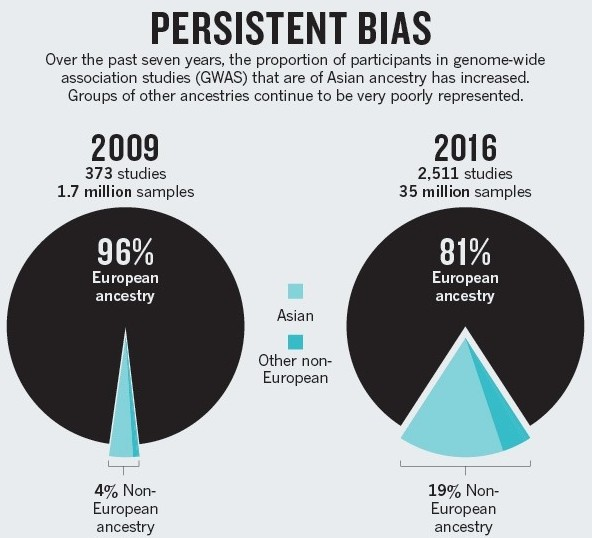
\includegraphics[width=0.6\textwidth]{GWAS-ancestry.jpg}}
\caption{Proportion of GWAS participants by ancestry. Most GWAS include mainly European people, some now include Asian people, but other ethnicities are still poorly represented. Source: \cite{popejoy2016genomics}.}
\label{fig:GWAS-ancestry}
\end{figure}

This lack of heterogeneity in inclusion of diverse populations has several problems. First,
there are some SNP ascertainment bias because SNPs that are more common are more likely to be discovered in GWAS so that discoveries in European tend to have larger frequencies than in other populations, due to the winner's curse. If effects have a frequency that is different between populations, using these effects naturally introduces some shift in PRS distributions for different populations.
Second, rare variants are missed in GWAS if they are specific to some population that is not included in the association study \cite[]{martin2019clinical}. Thus, this limit the predictive ability of PRS in different populations to the one(s) included in the GWAS.
Third, it is accepted that genotyped SNPs, or even imputed SNPs, that are discovered in GWAS may not be true functional SNPs (fSNPs) having an effect on disease susceptibility. Instead, GWAS are assumed to discover SNPs that tag fSNPs (tagSNPs), i.e.\ are correlated with fSNPs. 
Yet, LD may be different between populations so that a tagSNP can have a different correlation with the corresponding fSNP. Thus, effects of these SNPs can be different and are often diluted toward zero for populations not included in the GWAS \cite[]{carlson2013generalization}. 
In conclusion, for many reasons, magnitude and frequency of effects can vary considerably between populations, and these differences are larger when populations are more genetically distant such as African population with either European or Asian populations.
These differences in prediction between populations are two-fold (Figures \ref{fig:dist-shift} and \ref{fig:pop-pred}): distributions of PRS are shifted and prediction within each distribution is also reduced \cite[]{vilhjalmsson2015modeling,martin2019clinical}.

\begin{figure}[htpb]
\centerline{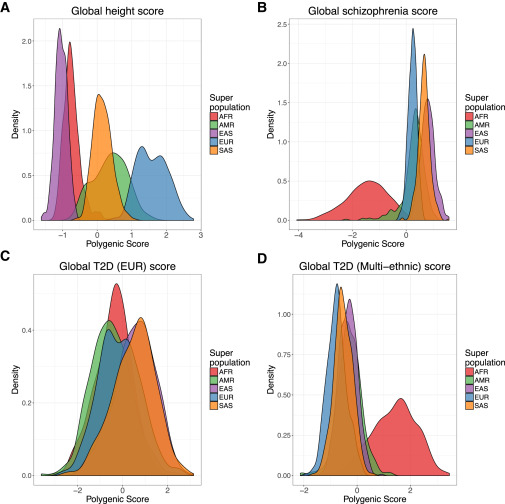
\includegraphics[width=0.6\textwidth]{pred-pops.jpg}}
\caption{Distributions of Polygenic Risk Scores (PRS) for many populations and phenotypes (T2D: type 2 diabetes). Source: \cite{martin2017human}.}
\label{fig:dist-shift}
\end{figure}

\begin{figure}[htpb]
\centerline{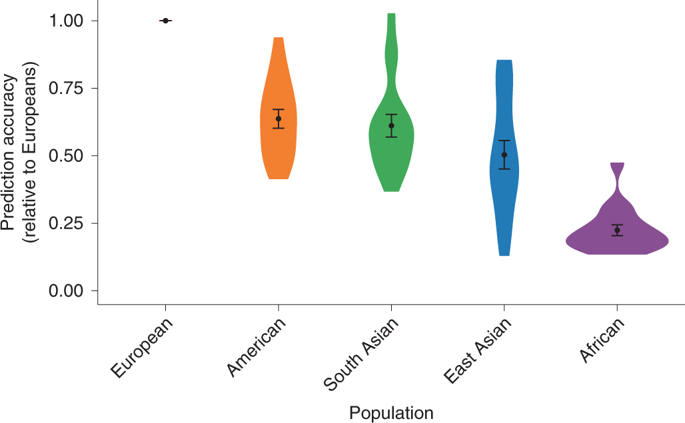
\includegraphics[width=0.7\textwidth]{pop-pred-reduced.png}}
\caption{Prediction accuracy relative to European-ancestry individuals across 17 quantitative traits and 5 continental populations in the UK Biobank data \cite[]{bycroft2017genome}. Source: \cite{martin2019clinical}.}
\label{fig:pop-pred}
\end{figure}


Several solutions have been proposed to partially correct for the differences of prediction between populations. First, \cite{martin2017human} proposed to mean-center PRS for each population, yet this would require an accurate way to assess ancestry and would not work for admixed people, e.g.\ one person with an African father and an European mother \cite[]{reisberg2017comparing}.
Second, it has been suggested to include more diverse population in GWAS \cite[]{pulit2010multiethnic}. Indeed, new associations can be found if the frequency is higher in an under-represented population. 
It would be also possible to fine-map fSNPs in common for multiple populations so that their effects generalize better to any population, irrespective of LD \cite[]{carlson2013generalization,finemap,wojcik2018page}.
Finally, statistical methods are being developed to use large European GWAS in conjunction with smaller data from another population in order to leverage both the discoveries from the large dataset and the specificities of the smaller dataset \cite[]{marquez2017multiethnic,coram2017leveraging}.


\subsection{Looking for missing heritability in rare variants}

Missing heritability, i.e.\ the gap between heritability estimations from current GWAS studies and from family studies, could reside in rare variants.
Indeed, for height and colorectal cancer, it has been shown that estimations of heritability from GWAS data could recover almost all heritability when a large proportion of low-frequency variants was present in the data \cite[]{yang2015genetic,huyghe2019discovery,wainschtein2019recovery}.
However, actual findings of significantly associated variants of low-frequency are scarce. 
For example, a GWAS of height including more than 700K individuals found 83 associated variants with allele frequencies between 0.1\% and 4.8\%, with effects up to 2 cm per allele \cite[]{marouli2017rare}. Yet, these 83 variants together accounts for only 1.7\% of the total heritability of height. 
In other large studies, one for coronary artery disease and one for type 2 diabetes, there was little evidence of low-frequency variants with large effects \cite[]{nikpay2015comprehensive,fuchsberger2016genetic}.

Associations of rare variants with traits are difficult to find for two reasons. 
First, it is very difficult to impute low-frequency variants with a good quality if using for example a small reference panel such as the 1000 genomes \cite[]{nikpay2015comprehensive}. There is now a reference panel of 32,000 individuals that is used to accurately impute variants with allele frequencies as low as 0.1\% \cite[]{mccarthy2016reference}. Ongoing large-scale projects, such as the Trans-Omics for Precision Medicine (TOPMed) programme, are expected to produce reference panels 
of more than 100,000 individuals \cite[]{taliun2019sequencing}.
This large reference panel is European specific, which means that imputing data from other ancestries is more difficult. This is a problem because, one way to discover and accurately estimate the effect of a rare variant is to look for it in a population in which its allele frequency is larger \cite[]{moltke2014common,minster2016thrifty}. 
Indeed, the power of association studies is dependent on the variance explained by a locus and its frequency; for example, for a disease that affects 1\% of the population, we have the same power to detect a risk locus of 50\% frequency and odds ratio of 1.1 as we do for a risk locus of 0.1\% frequency and odds ratio of 2.9 \cite{wray2018common}.

The second reason for which rare variant associations are difficult to find is that sequencing technologies are more expensive than genotyping and imputation. Currently, studies have mostly focused on whole exome sequencing (WES) because it is cheaper than whole genome sequencing (WGS). 
Indeed, the exome is where the effect sizes of variants are expected to be larger and where discoveries are likely to be more immediately actionable \cite[]{zuk2014searching}. 
Yet, sample sizes of sequencing studies remain small and special considerations and challenges arise when testing rare frequency variants from these studies \cite[]{auer2015rare}.
Thus, sample size is the limiting factor in variant discovery, not genotyping technology \cite{wray2018common}. 
It is probably the limiting factor in prediction too.

\subsection{Looking for missing heritability in non-additive effects}

Knowledge about biological pathways and gene networks implies that epistasis (gene interactions) might be important to consider \cite{hill2008data}. 
Apart from explaining missing heritability, genetic interactions could also create phantom heritability, i.e.\ could make current estimation of heritability upward biased \cite[]{zuk2012mystery}.
There have been some findings of interaction between loci, but mainly for autoimmune diseases where there are strong effects in regions of chromosome 6 that have an effect on the autoimmune system \cite[]{lenz2015widespread,goudey2017interactions}.
Yet, these interaction effects explain little to phenotypic variance as compared to additive effects \cite[]{lenz2015widespread}.
In general, data and theory point to mainly additive genetic variance \cite{hill2008data}.

Moreover, interactions are challenging to find for two reasons, and dedicated methods to epistasis detection have been implemented \cite[]{niel2015survey}. First, it is analytically impractical to search for such interaction effects because it would require testing more than 100 billion pairs of variants, even for a small genotyping array. Second, because of this huge number of tests, correction for multiple testing allows the detection of highly significant interactions only.

Finally, even if we find such interaction effects, they are unlikely to dramatically improve risk prediction for complex diseases, but could still provide insights into their ethiology \cite[]{aschard2012inclusion}. 
Moreover, due to differences in effect sizes and LD between populations, epistatic effects are even more unlikely than additive effects to replicate to different populations  \cite{hill2008data,visscher201710}.

\subsection{Integration of multiple data sources}

There are many genetic data out there. Some large individual-level data such as the UK biobank are available \cite[]{bycroft2017genome}. When GWAS data is not publicly available, summary statistics are often publicly shared instead. 
Usually, predictive models are based on either individual-level data (e.g.\ penalized regression) or summary statistics (e.g.\ C+T).
Building models that combine both individual-level data and summary statistics, possibly including different populations, is necessary to increase predictive power.
We started to do this by implementing the SCT method in our latest paper, where we combine several summary statistics based predictors using large individual-level data.
Alike with the adaptive lasso \cite[]{zou2006adaptive}, one could also think of penalizing SNPs differently in individual-level data methods, applying a penalization factor to each SNP based on their significance in external summary statistics.

Human diseases are inherently complex and governed by the complicated interplay of several underlying factors \cite[]{dey2013integration}.
For a trait or a disease, prediction based on genetic data only is ultimately capped by heritability.
Therefore, prediction must integrate other types of data if we want to predict beyond the limit of heritability (Figure \ref{fig:data-layers}).
For example, DNA methylation data can accurately predict age of any tissue across the entire life course \cite[]{horvath2013dna,horvath2018dna}, gene expression profiles enable to gain a broad picture of the genomic response to environmental perturbation \cite[]{gibson2008environmental} and microbiota can also be an important ``environmental'' factor to take into account \cite[]{backhed2004gut}. 
Yet, integrating variables with different formats, types, structure, dimensionality and missing values is a challenging problem \cite[]{dey2013integration}.
One could integrate genetic data with clinical data. For example, \cite{inouye2018genomic} designed a polygenic risk score (PRS) with higher discriminative ability for coronary artery disease than any of 6 conventional risk factors (smoking, diabetes, hypertension, body mass index, high cholesterol and family history).
Using this PRS with all 6 conventional risk factors increases discriminative ability as compared to using the PRS only or the 6 factors only.
Moreover, electronic health records (EHR) make possible to integrate large biobank datasets with large clinical, environmental and phenotypic information \cite[]{roden2016integrating}.
%Three different approaches for data integration are presented in figure \ref{fig:int-data} \cite[]{dey2013integration,zitnik2019machine}.

\begin{figure}[htpb]
\centerline{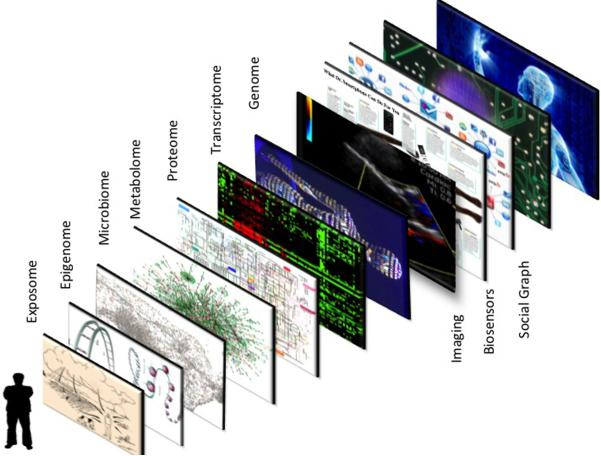
\includegraphics[width=0.7\textwidth]{data-layers}}
\caption{Geographic information system of a human being. The different layers of data available for an individual. Source: \cite{topol2014individualized}.}
\label{fig:data-layers}
\end{figure}


\subsection{Future work}

I will probably continue to work in the field of Predictive Human Genetics. I am currently visiting the National Center for Register-based Research (NCRR) in Aarhus, Denmark. Researchers there are mostly epidemiologists using some national registers where they have information on all Danes over decades. Most of their work is funded to look at psychiatric disorders and they are now interested in how genetics influence psychiatric conditions. It is a good opportunity to work on a large national biobank dataset with Bjarni Vilhj\'almsson.

I would be interested in looking at many things. 
First, I think investigating which method works best in which scenario is of great interest for the field. 
Many scenarios could involve different sample sizes of summary statistics and individual-level data, but also training and prediction in different populations.
Such work could be useful to make some guidelines about which method to use in which situation. For example, individual-level data methods often work best when large individual-level data are available, but what about predicting in a different population where only smaller datasets are available?
Second, it would be interesting to account for age in the prediction, for example extending with Cox regression the methods I implemented. Many diseases such as cancer, heart diseases and Alzheimer's disease have an age component; modeling this age component and accounting for right censoring (people who might develop disease later) should increase predictive performance and usefulness of models.
Third, I would like to investigate more about imputation. At the moment, imputed data is taken for granted. How to properly account for imputation accuracy in association testing (using e.g.\ multiple imputation) and in predictive models? 

Finally, other ideas could be to investigate how we can integrate many sources of information such as functional annotations, looking at many phenotypes at once, or to distinguish between two diseases with similar symptoms using polygenic risk scores (e.g.\ diabetes).

\newpage

\bibliographystyle{natbib}
\bibliography{refs}

\end{document}



\cleardoublepage
\phantomsection
\addcontentsline{toc}{chapter}{Bibliography}
\bibliographystyle{natbib}
\bibliography{refs}


\appendix

\chapter{Code optimization based on linear algebra}

\section{Lightning fast multiple association testing}.

In this section, I describe how to quickly test many variables for an association with a continuous outcome of interest. For example, let us make a Genome-Wide Association Study (GWAS) of height, i.e. we want to determine which genome variants are associated with height.

The model we want to test is $$y = \beta s + X \gamma + \epsilon~,$$ where $s$ is one variant (we want to do this for each variant, separately), $X$ are some covariates to adjust for some possible confounding factors (a matrix of $N$ samples over $K$ columns, including a column of $1$s to account for an intercept in the model). 
We are only interested in estimating $\hat{\beta}$ and computing a p-value corresponding to the significance of the alternative hypothesis that $\beta \neq 0$.

\cite{sikorska2013gwas} show that we can rewrite this problem as $$y^* = \beta s^* + \epsilon~,$$ where $y^* = y - X (X^T X)^{-1} X^T y$ and $s^* = s - X (X^T X)^{-1} X^T s$. Thus, this becomes a simple linear problem which is easy and fast to solve. We have
\begin{align*}
\hat{\beta} &= \dfrac{s^{*T} y^*}{s^{*T} s^*} \\
\widehat{\text{var}}(\hat{\beta}) &= \dfrac{(y^* - \hat{\beta} s^*)^T (y^* - \hat{\beta} s^*)}{(N - K - 1) ~ s^{*T} s^*} \\
\frac{\hat{\beta}}{\sqrt{\widehat{\text{var}}(\hat{\beta})}} &\sim T(N - K - 1)
\end{align*}

We go further by computing the singular value decomposition $X = U \Delta V^T$ ($N \times K$ matrix). As $N \gg K$, we have $U^T U = I_K$, $V^T V  = I_K$ and $V V^T = I_K$. Thus $X (X^T X)^{-1} X^T = U \Delta V^T (V \Delta U^T U \Delta V^T)^{-1} V \Delta U^T = U \Delta V^T (V \Delta^2 V^T)^{-1} V \Delta U^T = U \Delta V^T (V \Delta^{-2} V^T) V \Delta U^T = U U^T$.
We can simplify $s^{*T} y^* = (s - U U^T s)^T y^* = s^T y^* - s^T \underbrace{U U^T y^*}_0 = s^T y^*$, 
$s^{*T} s^* = (s - U U^T s)^T (s - U U^T s) = s^T s - 2 s^T U U^T s + s^T U U^T U U^T s = s^T s - s^T U U^T s = s^T s - z^T z$, where $z = U^T s$, 
and $(y^* - \hat{\beta} s^*)^T (y^* - \hat{\beta} s^*) = y^{*T} y^* - 2 \hat{\beta} s^{*T} y^* + \hat{\beta}^2 s^{*T} s^* = y^{*T} y^* - 2 \hat{\beta} s^{*T} y^* + \hat{\beta} s^{*T} y^* = y^{*T} y^* - \hat{\beta} s^{T} y^*$.
So, we only need to compute
\begin{align*}
z &= U^T s \\
\hat{\beta}_{\text{num}} &= s^{T} y^* \\
\hat{\beta}_{\text{deno}} &= s^T s - z^T z \\
\hat{\beta} &= \hat{\beta}_{\text{num}} / \hat{\beta}_{\text{deno}} \\
\widehat{\text{var}}(\hat{\beta}) &= \dfrac{y^{*T} y^* - \hat{\beta} ~ \hat{\beta}_{\text{num}}}{(N - K - 1) ~ \hat{\beta}_{\text{deno}}}~.
\end{align*}
Since $U$ and $y^*$ are computed only once for all variants, you can apply those formulas to compute these statistics for \numprint{1000000} variants and $N$=\numprint{500000} samples and $K$=$11$ covariates in one hour only \cite[]{prive2018efficient}. This is implemented in function big\_univLinReg() of package bigstatsr.


\bibliography{refs}


\afterpage{\blankpage}


\end{document}
